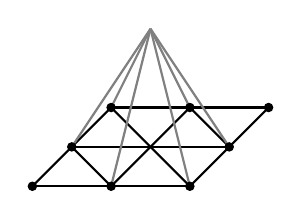
\begin{tikzpicture}[scale=0.25]

  % quad mesh lines
  \draw[thick] (0,0) -- (8,0);
  \draw[thick] (2,2) -- (10,2);
  \draw[thick] (4,4) -- (12,4);
  \draw[thick] (0,0) -- (4,4);
  \draw[thick] (4,0) -- (8,4);
  \draw[thick] (8,0) -- (12,4);

  % diagonals triangulating each quad (other orientation)
  \draw[thick] (4,0) -- (2,2);
  \draw[thick] (8,0) -- (6,2);
  \draw[thick] (6,2) -- (4,4);
  \draw[thick] (10,2) -- (8,4);

  \def\ytop{8};

  % ridge lines from tent peak to 6 surrounding nodes
  \draw[gray,thick] (6,\ytop) -- (4,0);
  \draw[gray,thick] (6,\ytop) -- (8,0);
  \draw[gray,thick] (6,\ytop) -- (2,2);
  \draw[gray,thick] (6,\ytop) -- (10,2);
  \draw[gray,thick] (6,\ytop) -- (4,4);
  \draw[gray,thick] (6,\ytop) -- (8,4);

  % nodes in base plane
  \filldraw (0,0) circle (6pt);
  \filldraw (4,0) circle (6pt);
  \filldraw (8,0) circle (6pt);
  \filldraw (2,2) circle (6pt);
  %\filldraw (6,2) circle (6pt);   % (x_p,y_q) is at (6,2), shown at tent top
  \filldraw (10,2) circle (6pt);
  \filldraw (4,4) circle (6pt);
  \filldraw (8,4) circle (6pt);
  \filldraw (12,4) circle (6pt);
\end{tikzpicture}
